\section{Experimental Setup}\label{sec:experimentalSetup}

In this section, we describe how to setup our study. We first describe how we mined the data-set of Android app pairs that will serve as a benchmark for our study.Then we enlist and justify the test generation tools that mine for android sandboxes. Then, we describe the setup of our infrastructure used to perform the study. 

\subsection{Dataset}
\textbf{Collect apps pair (benign-malicious).} Most malware are simply repackage of official app where repackage app injects an extra code, often malicious, to original apps. Zhou et al.~\cite{DBLP:conf/sp/ZhouJ12} provided a wide-ranging malware collection, where 80\% of samples are know to be built by repackaging other apps. Because of this our dataset is composed by app pairs (benign-malicious).

%\kn{Here we need one or two lines motivating why we need app pairs.} 

To populate our app pairs, we used Androzoo~\cite{DBLP:conf/msr/AllixBKT16}, a collection of Android apps mined from multiple markets, including the official Google Play~\footnote{\url{https://play.google.com/store}}. Androzoo makes an ideal source of apps as it was designed with a primary goal of aiding research studies such as ours. 

Due to space and time constraints, we downloaded 42 GB of apps for 20 hours and ended up with 7268 app pairs. Androzoo sometimes contains multiple malicious versions for the same benign app. In such cases, we pick the first malicious version ensuring that the resulting pairs were unique in terms of their original apps. This step resulted in our dataset containing 1831 app pairs. Among 1831 initial pairs, only 1395 apps could be successfully instrumented by DroidFax. Among the 1395 instrumented pairs, we had installation errors on our emulator (Pixel 4 API 28), many times due to compatibility issues. 

In all, we obtained 824 valid app pairs that could be used for our study. Figure~\ref{fig:stores} presents the markets where the most of malicious version apps were collected according to Androzoo. As we can see, even at the official Google Play market, it is possible to extract several malware.
%\kn{TODO: Convert Table 1 into a bar chart listing only the top 6. The rest of the app stores with less than 10 apps can be listed in the appendix } 


\begin{figure}[ht]
\centering
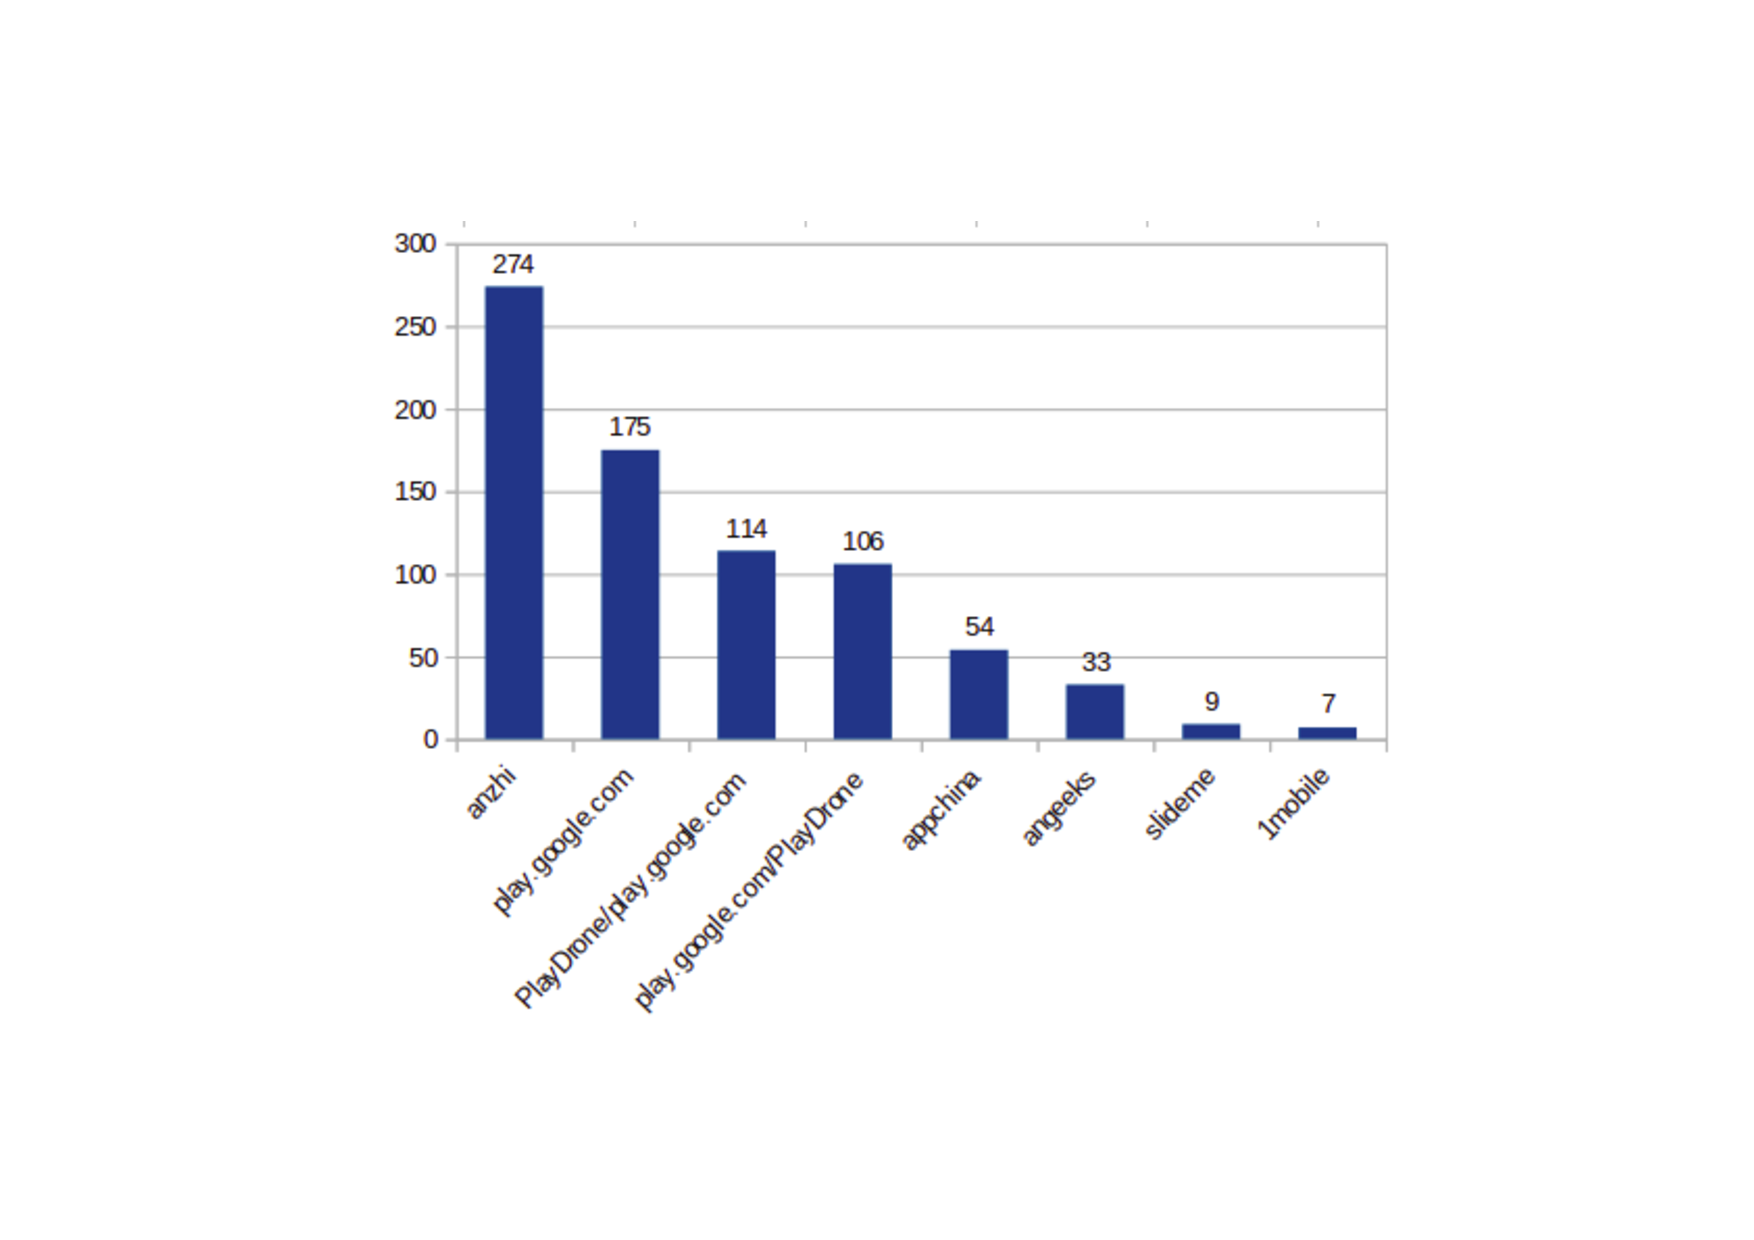
\includegraphics[scale=0.32]{images/stores.pdf}
\caption{Markets where malware was downloaded.}
 \label{fig:stores}
\end{figure}

To perform an in-depth analysis of how various factors influence the quality of android sandboxes, we utilize four state of the art test generation tools: Monkey~\cite{Monkey}, Droidmate2~\cite{DBLP:conf/kbse/BorgesHZ18}, Droidbot~\cite{DBLP:conf/icse/LiYGC17} and Humanoid~\cite{DBLP:conf/kbse/LiY0C19}. We considered Monkey because it is part of the Android SDK, easy-to-use, and compatible with different Android versions. It is also the most widely used randomly test generation tool for Android in industry~\cite{DBLP:conf/sigsoft/ZengLZXDLYX16}. 

We choose Droidmate2, an enhancement of the Droidmate~\cite{DBLP:conf/icse/JamrozikZ16} project, as it is a state of the art in harnessing random screen actions such as long-clicks, swipes etc. to invoke GUI elements in an app. 

Droidbot is another test generator tool in our study that applies a depth-first strategy (DFS)~\cite{DBLP:conf/oopsla/AzimN13} to dynamically build  GUI models collecting GUI information and running process
information. Droidbot achieved better performance results when mining sensitives resources in comparison with the state of the art\cite{DBLP:conf/wcre/BaoLL18}~\cite{DBLP:journals/jss/CostaMMSSBNR22}. 

In order to react to the advancements in the field of AI for malware detection, we also used Humanoid~\cite{DBLP:conf/kbse/LiY0C19}, a deep learning-based tool that emulates realistic users, creating human-like test inputs. Humanoid implements a deep neural network model that learns which UI elements an Android user interacts with and how. It is built on Droidbot and has shown to have better code coverage when compared to others test generator tools.


\subsection{Mine Android Sandbox Infrastructure}

For our study, we require an extensive infrastructure that will allow us to integrate different test case generation tools. To this end, we used and extended DroidXP\cite{DBLP:conf/scam/CostaMCMVBC20}, a benchmark tool that allows researchers and developers, to integrate and compare test case generation tools for mining sandboxes.

Using DroidXP, test case generation tools can be integrated and deployed easily~\footnote{The DroidXP benchmark is available at https://github.com/droidxp/benchmark}. Another reason to use DroidXP is that it relies on DROIDFAX~\cite{cai2016understanding}, which allowed us to instruments Android apps and collect important information about their execution. For example, this can be used to query for the calls to the sensitive APIs from an app during executions which is important to monitor malicious behavior. 

%\kn{I have commented out the following and shortened it as this is too verbose information about DroidXP's tooling}
\begin{comment}
The DroidXP relies on a Simple Command Line (CLI) that  provides commands for execution of different experiments with several setup, following parameters:
\newline
\newline
\textbf{DroidXP:} python main.py [-h] [--list-tools] [-tools] toolName [-t] timeSeconds [-r] repetition [--list-outputs] [--output] output [--debug] [--version]\newline
\newline
One can show help message [-h], list available test generation tools [--list-tools], test tools used in the experiment (toolName), threshold of the execution time in the experiment (timeSeconds), number of repetitions used in the experiment (repetition), list available output formats [--list-outputs], output formtat that will be used to show results (default: basic) (output),
run in DEBUG mode (default: false) [--debug] and print DroidXP version [--version].

Follow an example of a command line that executes DroidXP for three minutes (180 seconds), at test generation tools Monkey, repeating all the performance three times, and outputting the final result at a CSV file format:
\newline
\newline
\textbf{python main.py -tools monkey -t 180 -r 3 --output csv}
\newline
\end{comment}


Benchmarking using DroidXP typically happens in three phases:

\textbf{Phase 1: Instrumentation:} In the first phase, a set of APK files is provided as input to DroidXP. This set is composed by all the app pairs (benign/malicious) used at our study. Each APK file is then instrumented to be able to collect data about the execution. This instrumentation is performed by DroidFax. To improve the performance, the set of pairs already instrumented are available, so it's not necessary to spend too much time instrumented the same pairs in multiple executions. In this phase, each app is statically analyzed to collect the number of methods and classes inside the app, which is necessary to measure coverage during execution. %\kn{I dont understand this statement, which set are pre-instrumented, whats the instrumentation like, who defines this set}. 

\textbf{Phase 2: Execution:} In this phase, the execution is done by deploying an instrumented APK file in an Android emulator and executing the instrumented app using one or more test generation tools for a chosen period of time. To ensure that each execution gets the benefit of running on a fresh android instance without biases that could stem out of history, all data stored on the emulator from previous executions are wiped out from the emulator. 

%\kn{Is the result analysis into logcat done by DroidXP or an extension by us? In general, it is unclear what is existing in DroidXP already and what we do. Isnt logcat a separate tool. If this is done by DroidXP, please make it clear that DroidXP invokes logcat on its own}%
\textbf{Phase 3: Result Analysis:} During the execution, all the data that is required to compute the results are persisted by DroidXP, using Logcat \cite{Logcat}, one of the Android SDK's native logging tools. This can be used to perform analysis on the results of executing test generators on apps and observe malicious behavior. 

\textbf{DroidXPTrace}. To leverage our study, we also used an auxiliary tool from DroidXP project called DroidXPTrace~\footnote{The DroidXPTrace is also available at https://github.com/droidxp/droidxptrace}. DroidXPTrace allowed us to monitor aspects like dynamic call graphs which was not possible using vanilla version of DroidXP. DroidXPTrace, using the result from Phase 3 of DroidXP, creates a call graph of app pair, exploring traces from its entry point to sensitive API access. In the end, it compares both call graphs (benign and malicious app version), and generated a JSON file recording the following information:
%\kn{I have rephrased the previous paragraph, please check if it is still accurate}. 

%\kn{Overall the following bits in the rest of this subsection are a bit confusing.  You use the word trace and graph interchangeably. is it a graph or a trace. And finally the connection to paths taken comes out of nowhere. I propose rephrasing this part with an example data from some app. Only one of the columns is enough. Even if the example is an artificial one it is fine. Important is that it becomes clear what data is recorded. }
\begin{itemize}
\item \texttt{benign}: Name of log file from the benign app version
\item \texttt{malign}: Name of log file from the malicious app version
\item \texttt{benignGraphs}: call graphs that contain traces with access to sensitive methods in the benign version of the app.
\item \texttt{malignGraphs}: call graphs that contain traces with access to sensitive methods in the malicious version of the app.
\item \texttt{methodsAccessedOnlyByMalign}: The sensitive methods that are accessed only by the malicious version of the app. This information is important to identify if a particular sensitive call that is undetected by a sandbox occurs only in a malicious version.
\item \texttt{benignGraphContainsMalignGraph}: Comparison between benign and malicious sub-callgraphs
\item \texttt{hasDifferentTraces}: whether the benign and malicious app version have different traces to sensitive resources. 
\end{itemize}

Thus, we added additional information of call graphs at our study. This information helped us to explore traces between an entry point app and its access to methods sensitives, at runtime. This investigation shows that in several situations, although both app versions (benign-malicious) access the same set of sensitive resources, they access them using different traces, which could mean malicious sensitive resource access.

\subsection{Hardware and procedure setup}

We deployed our experiment on a machine running a 64-bit Debian  GNU/Linux 11. The machine used was  a 32-Core, AMD EPYC 7542 CPU, 512 GB RAM, storage Samsung SSD 970 EVO 1TB. We also configure our emulator to run all selected apps on Google Android version 9.0, API 28, 512M SD Card, 7GB internal storage, with X86 ABI image.

For our study, we configured DroidXP to run each of the 824 app pairs using each testing tool for three minutes. To mitigate noise, we repeated the full process three times which took in total ($824 \times 2$ apps $\times 4$ tools $\times 3$ runs $\times 3$ min $\apeq 989$ machine hours).
%\kn{Initial? Was there a follow up study, if not please use only study. This is feedback for all instances with the word initial}

Although it was possible to run more than 10 emulators in parallel on one physical machine, to avoid any interference due to context switching within the operating system, we choose to run one emulator at a time. Hence, all evaluation processes took around 41 days and additional five days for environment deployment.

In the following subsections, we describe the setup required to perform custom analysis that were central to our study. 
\subsection{Similarity analysis} \label{sec:similarity}

To validate the impact of repackaged apps for sandbox approaches, we perform a \textit{similarity analysis} of the app pairs using SimiDroid~\cite{DBLP:conf/trustcom/0029BK17}. It quantifies and qualifies the similarity between pair following four metrics that is considered most relevant~\cite{DBLP:conf/wcre/0029BKT16}. The four metrics are primarily based on method level differences:

\begin{itemize}
    \item \textit{identical}: a given method is considered identical if both versions have the same signature and the same implementation
    \item \textit{similar}: a given method is similar if both versions have the same signature but not the same implementation.
    \item \textit{new}: a given method is new if it is present only in the malicious version of the app.
    \item \textit{deleted}: a given method is deleted if it is present only in the benign version of the app.
\end{itemize}

Based on these metrics, SimiDroid computes the similarity score of the given app pairs using Formula\eqref{eq:1}.

\begin{equation}
 similarity = max \lbrace\frac{identical}{total-new},\frac{identical}{total-deleted}\rbrace  \label{eq:1}
\end{equation}

where

\begin{equation}
 total = identical + similar + deleted + new\label{eq:2}
\end{equation}
\newline
Our similarity analysis was important for our experiment since it allowed us to check how similar or different are the pairs in terms of code content. With this information, we could check which strategies for malware detection are more effective when given pairs are very similar. Previous state of the art work \cite{DBLP:conf/codaspy/ZhouZJN12} limited their study of repackaged app detection by setting a similarity threshold of 70\%. In our study, we do not filter any of the select app pairs with any threshold criteria, since our idea is to present a fine-grained analysis of the relationship between app similarity and the ability of different sandbox approaches to detect them.

\subsection{Manifest file analysis}\label{sec:manifestAnalysis}

Our work also observed the Manifest file of all app pairs. These files present essential security information which the Android system must know before executing an app. Among other things, a  list of requested permissions and a list of important components are persisted in the manifest file. Unfortunately, Manifest files are generally not considered by sandbox approaches when detecting malware inspite of the fact that they can are easily modified by malicious developers~\cite{DBLP:journals/corr/abs-1208-4536}. For instance by inserting new permission requests or component capabilities (actions). Such injections can happen either manually or through automated scripts.

Automated process sometimes generate Manifest file with duplicate permission requests, as the original app may already contain the permission request. Such duplication happen with actions too (e.g., where to transfer the ad revenues). On top of this, our manifest analysis also allowed us to monitor suspicious new permissions or excessive amounts of permissions. 

To extract and analyze the Manifest file, we used an in-house Android SDK analyzer called \textit{apkanalyzer}. We implemented a python script that using \textit{apkanalyzer}, computed which malicious apps had duplicated request permission or duplicated actions. The script also extracted how many permissions were requested by all apps, in both versions, to help us monitor suspicious features. Listing~\ref{lst:androidManifestDupli} presents an example of duplicated permission extracted from malicious version of the app \textbf{com.ifeel.frogjump}. The listing suggests that the four first requested permission could have been added automatically as part of a naive hacking script.
%\kn{app-8 according to what table? reference please}. 

\begin{lstlisting}[caption={Example of duplicated permission from malicious version of app com.ifeel.frogjump}, language=Java,
    basicstyle=\fontsize{6}{5}\selectfont\ttfamily,
    label={lst:androidManifestDupli}]

13:M >  <uses-permission
        android:name="android.permission.READ_PHONE_STATE" />

16:M >  <uses-permission
        android:name="android.permission.ACCESS_COARSE_LOCATION" />

19:M >  <uses-permission
        android:name="android.permission.INTERNET" />

22:M >  <uses-permission
        android:name="android.permission.ACCESS_NETWORK_STATE" />
    .
    .
    .
134:M > <uses-permission
        android:name="android.permission.INTERNET" />

137:M > <uses-permission
        android:name="android.permission.WAKE_LOCK" />

140:M > <uses-permission
        android:name="android.permission.READ_PHONE_STATE" />

143:M > <uses-permission
        android:name="android.permission.ACCESS_NETWORK_STATE" />

146:M > <uses-permission
        android:name="android.permission.WRITE_EXTERNAL_STORAGE" />

149:M > <uses-permission
        android:name="android.permission.ACCESS_WIFI_STATE" />
\end{lstlisting}